\documentclass[12pt,a4paper]{article}

\usepackage{amsmath}
\usepackage{amsfonts}
\usepackage{amsthm}
\usepackage{mathtools}
\usepackage{hyperref}

% Personal Desktop
 \newcommand{\pathcommon}[1] {F:/latex_commons/#1}

% Heriot-Watt PC
% \newcommand{\pathcommon}[1] {C:/Users/jc2021/Documents/GitHub/latex_commons/#1}

\newcommand{\dobibliography} {\bibliographystyle{apalike} \bibliography{\pathcommon{bibliography}}}
\input{\pathcommon{standard_theorems}}
\input{\pathcommon{derivatives}}

\newcommand{\realfunction}[2] {{#1: #2 \rightarrow \mathbb{R}}}
\newcommand{\uexp}[1] {{\text{uexp}_{#1}}}

\title{Fitting absolutely monotonic functions}
\author{Juan Casanova}

\begin{document}

\maketitle

This is the abstract.

\tableofcontents

\section{Introduction}

This paper has two purposes. First, to present a method for fitting absolutely monotonic functions to data. Second, to discuss in this context three areas of mathematics research that, surprisingly, are rarely discussed together. We summarize the relevant similarities and connections of each of them with the aforementioned method, and consequently between them, as well as how this relates to potential applications of this work and existing literature.

\subsection{Absolutely monotonic functions}

A smooth function $\realfunction{f}{[a,b]}$ (where $b$ can be $+\infty$) is {\emph{absolutely monotonic}} if all of its derivatives are non-negative at every point in the interval. A simple example of an absolutely monotonic function is the exponential $e^x$, and in fact in a very significant sense, it can be shown that all absolutely monotonic functions are essentially sums of exponentials, a key idea supporting this work. More accurately, in his classic work \cite{1929_bernstein_absolutely_monotonic}, among other things, Bernstein characterized all absolutely monotonic functions as weighted averages of exponential functions with positive exponents.

\begin{theorem}[\cite{1929_bernstein_absolutely_monotonic}]
\label{bernstein_theorem}
Let $\realfunction{f}{[a,b]}$ (where $a$ and $b$ are both finite) be an absolutely monotonic function. Then, there is a non-negative finite Borel measure $\mu$ such that

\begin{equation}
f(x) = \int_{0}^{\infty} e^{tx} d \mu(t)
\end{equation}

\noindent for every $x \in [a,b]$.
\end{theorem}

There is a direct connection between absolutely monotonic functions and {\emph{completely monotonic functions}}, which are smooth functions with alternating sign derivatives. Specifically, a function $f(x)$ is absolutely monotonic in $[a,b]$ if and only if the function $f(-x)$ is completely monotonic in $[-b,-a]$. For example, $e^{-x}$ is a completely monotonic function, and similarly, Bernstein's theorem, when applied to completely monotonic functions, characterizes them as weighted averages of exponential functions with negative exponents (the Laplace transform of the non-negative measure $\mu$).

In informal terms, one can describe the function $e^x$ to be absolutely monotonic {\emph{towards the right}} and completely monotonic {\emph{towards the left}}, and the absolutely monotonic or completely monotonic views of functions are more related with what side of the function we are focusing on, and the corresponding properties that they have on them.\\

For various significant reasons, there has been substantially more work on completely monotonic functions than on absolutely monotonic functions. While it is tempting to argue that they are simply two sides of the same coin, their relation is limited by the nature of the result we are focusing on. More precisely, a lot of the work on completely monotonic functions considers them in the half-line $[0,\infty)$, which when mirrored results in the interval $(-\infty,0]$ for absolutely monotonic functions. However, the interesting monotonic behaviour of absolutely monotonic functions is most relevant in intervals on the right side of the real line. Similarly, completely monotonic functions involve small absolute values and controlled decay, whereas absolutely monotonic functions involve very large absolute values and unfettered growth. This means that the types of interesting behaviours and challenges in each of these two sides of the coin can be quite different in practice.\\

Absolutely monotonic and completely monotonic functions are particular cases of exponential sums. When both positive, negative, and complex exponents are combined, more general types of functions appear, including periodic functions and variations on these.\\

Absolutely monotonic functions form a {\emph{convex cone}}. In particular, weighted sums of absolutely monotonic functions are absolutely monotonic.

\begin{lemma}
If $f, g$ are absolutely monotonic functions and $\alpha, \beta \in [0,+\infty)$, then $\alpha f + \beta g$ is an absolutely monotonic function.
\end{lemma}

The proof is trivial by looking at the definition of absolute monotonicity in terms of non-negative derivatives and linearity of derivation.

This can naturally be extended to infinite sums of functions (of which the Bernstein theorem presents a particular case) over non-negative measures, but we will not use this result in this work so we skip the proof of this slightly more general result. Other than Bernstein's theorem, we will limit ourselves to finite sums of absolutely monotonic functions.\\

We do not concern ourselves too much with further theoretical properties of absolutely monotonic or completely monotonic functions in this work, but for the interested reader, \cite{2014_koumandos_completely_monotonic} offers a modern summary of theoretical results and additional related families of functions, such as logarithmically completely monotonic functions, Bernstein functions, and Stieltjes functions.\\

\cite{2011_rajba_integral_representation_convex_functions} is a particularly interesting piece of work partially bridging the gap between methods focused on convexity and absolute monotonicity. It presents an integral representation of {\emph{$n$-convex}} functions, which are functions where a certain number of derivatives are positive. In other words, an absolutely monotonic function is a function that is $n$-convex for every $n$. The mathematics in this work and the representation it offers for $n$-convex functions are strongly reminiscent of the Bernstein theorem. In particular, there is a direct relationship between the terms in this work and the Taylor series of the exponential function, indicating that this integral representation is using ``limited exponential functions'' consisting of partial Taylor series of exponential functions, up to the derivative that is required. It is surprising, then, that the work does not mention the Bernstein theorem or the words ``absolutely monotonic'' or ``completely monotonic'' whatsoever, or cite any work in this subject. More precisely, theorem 2.1 in \cite{2011_rajba_integral_representation_convex_functions} states that any n-convex function $f$ with regular derivatives in $(a,b)$ is such that:

\begin{equation}
f(x) = \int_{(a,\epsilon]} (-1)^{n+1} {{[-(x-u)]^n_{+}} \over {n!}} dg_{(n)-}(u) + \int_{[\epsilon,b)} {{(x-u)^n_{+}} \over {n!}} dg_{(n)+}(u) + Q(x)
\end{equation}

\noindent (with certain constraints on the terms in this equation).

Informally, one can draw a clear connection between this and absolutely monotonic and completely monotonic functions when we notice that ${{(x-u)^n_{+}} \over {n!}}$ is the truncated Taylor series for $e^x$ up to $n$, and therefore this equation is essentially separating the n-convex function $f$ into a completely monotonic part (to degree $n$), an absolutely monotonic part (to degree $n$), and a remainder term $Q(x)$ with lesser degree.

While we do not use them in this paper, this work can be relevant in extending some of the notions here to less constrained cases like $n$-convex functions, or to better understand the methods and their limitations.\\

\subsection{Fitting exponential sums}
\label{exponential_sums}

There is a large body of work on fitting exponential sums to data. A lot of this work is related to signal analysis and therefore is concerned with general exponential sums, including positive, negative, and complex terms; though practical work is often limited to discrete sums.\\ 

One of the most significant families of methods for fitting exponential sums are the so-called Prony methods. Prony methods are spectral methods that use the relation between exponential sums, uniform sampling, and difference equations that enable a certain type of frequency analysis using linear algebra. \cite{2021_keller_prony_methods} offers a modern survey of Prony methods, focusing on common principles, such that they are linear methods on the space of operators on functions, and that they rely on sampling at specific distances to capture periodic behaviours in the signals. A lot of work on Prony methods is related to the optimization of the linear algebra aspects of the algorithms.

Prony methods are more general in its function space, present more constraints to the data, and focus more on frequency analysis of a signal than on good numerical fitting of a real function. Their goal is the analysis of signals, often assumed to be in the $[0,+\infty)$ half-line, rather than the fitting of observed real data on the absolutely monotonic side of the function. Therefore, they are not particularly well suited for fitting absolutely monotonic functions, even if they could theoretically be applied. It could be interesting to apply some of these methods to examples on absolutely monotonic functions in bounded intervals by mirroring them and using Prony methods, to compare with the results in this paper, but we have decided not to pursue this avenue further.\\

Other methods have been explored for fitting exponential sums over time. \cite{1976_kammler_approximation_completely_monotonic} presents a theoretically focused and exploratory analysis of using Chebyshev polynomials to approximate completely monotonic functions. \cite{1976_smith_decomposition_exponential_decays} discusses several potential methods, also with a focus on completely monotonic functions, with limited success, and with significant computational constraints that are not applicable in the current time. \cite{1980_evans_least_squares_exponential_sum} uses a least squares algorithm to fit completely monotonic functions, but also suffers from being computationally obsolete. It does note, however, that with a least squares approach, numerical aspects become critical, such as initialization of values or behaviour of the parameter space. We will discuss these aspects later in this work. In a slightly more modern survey, \cite{2002_holmstr_parameter_estimation_fitting_exponentials} discusses a wide array of methods for fitting exponential sums, including Prony methods, least squares approaches, and many others. None of these pay significant attention to absolutely monotonic functions.

There is definitely room for further exploring whether some of these methods may be applied successfully with a focus on absolutely monotonic functions, but work would be required to adapt them. We believe that between the focus on complex exponent signals, completely monotonic functions, the differences in error measurements between fitting a slow decay function and a fast growth function, and the outdated computational considerations of some of the older pieces of work, making any of these methods work successfully on absolutely monotonic functions would not be straightforward. Moreover, the method presented in \S \ref{method} uses a least squares approach with a specific choice of representation of exponentials that improves numerical behaviour of the optimization algorithm, resulting in a very simple and relatively fast algorithm that gives significantly satisfying results. This suggests that there is no need to painfully adapt methods designed for other problems when a relatively simple one exists for this problem. It would, however, be interesting to verify this with an actual comparison.

\subsection{Fitting monotonic and convex functions}

The methods discussed in \S \ref{exponential_sums} are parametric or semi-parametric, using a predetermined family of functions and fitting using parameterizations. This ensures certain properties of the resulting fit by construction (complete monotonicity, periodic behaviour, etc). Another family of work focuses instead on fitting the data accurately while imposing the desired properties in less constructive ways. Specifically, we are talking about the wide range of work on fitting monotonic or convex functions in general.\\

Absolute monotonicity is a particular case of convexity, which is a particular case of monotonicity. Absolute monotonicity is a stronger constraint. Two important questions deserve to be explored. First, can methods to fit monotone or convex functions be extended to absolute monotonicity constraints? Second, since absolutely monotonic functions are convex, can methods constrainted to absolutely monotonic functions be used when the target constraint is weaker (convexity)?\\

All or most of the work in this area expresses the fit as an optimization problem (e.g. linear programming), that minimizes the error, and uses additional constraints on the optimization problem and/or steps in the algorithm to ensure the monotonicity/convexity of the result. They are all heavily focused on local properties of the functions and how to encode the constraints in this way, e.g. by looking at properties of derivatives/gradients/jacobians/hessian matrices.

We found two major families of research. First, work on imposing monotonicity constraints to splines. Second, fitting convex functions in a multivariate context.\\

A {\emph{spline}} is a smooth piecewise polynomial. Spline interpolation is widely used because it is simple, very efficient, and produces smooth satisfying results for interpolation. However, while splines are smooth by design, imposing monotonicity in them is not easy. Work like \cite{1998_he_monotone_spline,2004_zhang_monotone_splines, 2013_nagahara_monotone_splines_linear, 2015_lu_spline_monotonic_regression} considers a candidate spline interpolation, and defines a linear programming problem that minimizes its error with respect to the data. It then introduces the monotonicity constraint as additional constraints on the linear program. The results are satisfying but limited, because imposing monotonicity on splines can severely affect their ability to adequately approximate the data, or the constraints may not be strict and may result in functions that are not monotonic at every point. Moreover, extending this to absolutely monotonic functions seems extremely hard, since new ways of representing the constraints on all derivatives of absolutely monotonic functions in a linear program would need to be devised, without significantly affecting the computational and approximation properties of the resulting algorithm.\\

Work like \cite{2013_hannah_multivariate_convex_regression} considers the more general problem of fitting convex multivariate functions to data. Particularly due to the multivariate nature, this problem is significantly more complicated. Various techniques are used to balance the convexity constraints with the goal of a good fit to the data. For example, \cite{2005_lachand_minimizing_convex_bodies} uses a projection step as part of a gradient descent algorithm to ensure the solutions are convex, while \cite{2008_aguilera_approximating_optimization_convex_functions} focuses on finding local characterizations of convexity and discretization of the hessian matrix of the target function, to ensure the convexity of the solution. These solutions are significantly computationally expensive, and struggle with balancing difficult constraints in a large solution space, due to their multivariate nature. Moreover, while convex but not absolutely monotonic functions are more rare, the application space is still more limited than our target problem.

It might be worth comparing the performance, in computational cost and goodness of fit, of these solutions to our proposed method for the problems in which they overlap (monotonic and convex functions). We expect these will be more cost for worse fit.\\

\subsection{Why absolutely monotonic functions}

Monotonic and convex functions are much more general than absolutely monotonic functions. Similarly, exponential sums appear in signal and frequency analysis, and completely monotonic functions can be relevant in economic modeling. These applications, and the lack of a comparatively as significant volume of applications for absolutely monotonic functions, explain the differences in the volume of work devoted to them. Why, then, do we want to fit absolutely monotonic functions? While this paper is focused on the method, we arrived at this problem from an applied setting. We wanted to use data to fit reward functions (for players in a video game). Absolute monotonicity is an extremely attractive constraint for a reward function, as it ensures not only that better results produce better rewards, but also that the returns increase, as it is often informally said, {\emph{exponentially}}, or more accurately, absolutely monotonically. This means that the same comparative improvement in performance will always result in a larger improvement (and a faster increase in this improvement, and a faster increase on the speed of this improvement, etc.) on the reward the higher the performance already is. In other words, small differences become much more noticeable near the top, which is very attractive for reward functions, for example in a competitive setting. Another way to look at this is that an absolutely monotonic function is a way to re-scale a performance value into a reward space that is ``exponential'', greatly accentuating differences at higher performance value while giving less relevance to differences at lower performance values.\\

Naturally, convex functions are often enough to represent this type of behaviour. While we have not thoroughly explored the economics literature in search for uses of convex functions, we conjecture that there might be some applications in economics in which convex functions are expected, that would benefit from using absolutely monotonic functions instead, by giving them stronger reward behaviours. Moreover, the method discussed in \S \ref{method} is simple, fast, and successful enough that it might be used in place of other methods focused on convexity.\\

As a whole, we believe that any real-world modeling of a function that benefits from consistently accentuating differences at higher values, but fit this function using existing data, such as reward functions, could benefit from imposing an absolute monotonicity constraint on the result and using the fitting method described in this paper.

\subsection{Summary}

In the field of mathematical analysis there is a significant theoretical understanding of absolutely monotonic functions, completely monotonic functions, exponential sums in general, and other related families of functions. At the same time, several methods of fitting some families of exponential sums to data exist, coming primarily from the signal analysis world. This applied work often does not use the existing theoretical results to their full extent, and sometimes fails to recognize the connection between the different families of exponential sums and their properties. At the same time, another significant research field studies algorithms to fit monotonic and convex functions, without acknowledging their relation to absolutely monotonic functions, and therefore exponential sums, and therefore not attempting (semi-)parameteric approaches to this problem, that could benefit from easier to fulfill constraints, and better computational performance and fitness.\\

In the remainder of this paper we discuss our proposed, simple method for fitting absolutely monotonic functions that sits in the middle of all of this, and that could help as an initial step towards briding these gaps. Regardless of this new method, we believe it would be in the best interest of researchers in each of these fields to explore the results in each other's fields and consider how they might improve their approaches or reconsider some assumptions or choices that they make.

\section{Method}
\label{method}

In this section we describe the method that we use to solve the following problem:

\begin{problem}
Given a set of data points $\mathcal{D} = \{(x_i,y_i)\}$, we wish to fit an absolutely monotonic function $f$ to minimize the error between the $\{y_i\}$ and $\{f(x_i)\}$.
\end{problem}

Note that we do not prescribe the measure of error in the general definition of the problem, as that can be arbitary. We also are not looking at the strict definition of {\emph{minimize}} but rather a best effort approach to it. In general, this is the larger problem we are trying to address.

However, in this work we use a semi-parametric least squares optimization, which means that we are minimizing the mean squared error, and we use an iterative method to find a best effort solution within a prescribed family of functions. Further details are described in the remainder of this section. This is a consequence of our chosen method.

\subsection{Domain}

Since the data $\mathcal{D}$ is finite, there will be bounds on the $\{x_i\}$
\begin{equation}
\begin{array}{l}
a = \min x_i\\
b = \max x_i\\
\end{array}
\end{equation}

Therefore, we can safely constrain ourselves to absolutely monotonic functions $f: [a,b] \rightarrow f([a, b])]$. Moreover, we can reduce the problem to absolutely monotonic functions $\bar{f}: [0,1] \rightarrow f([a,b])$ through a simple affine transformation. By transforming the $\{x_i\}$ into $\{\bar{x_i} = {{x_i - a} \over {b - a}}\}$, if we have a solution $\bar{f}: [0,1] \rightarrow f([a,b])$ for the problem associated to $\{\bar{x_i}\}$, we can define

\begin{equation}
f(x) = \bar{f}({{x - a} \over {b - a}})
\end{equation}

\noindent and we have:

\begin{equation}
\begin{array}{l}
f(a) = \bar{f}({{a-a} \over {b-a}}) = \bar{f}(0)\\
f(b) = \bar{f}({{b-a} \over {b-a}}) = \bar{f}(1)\\
\end{array}
\end{equation}

\noindent (correspondence of bounds)

\begin{equation}
{f(x_i)} = \bar{f}({{x_i - a} \over {b-a}}) = \bar{f}(\bar{x_i})\\
\end{equation}

\noindent (correspondence of data points)

\begin{equation}
\nderiv{f}{n}(x) = {({{1} \over {b - a}})}^n {\nderiv{\bar{f}}{n}} ({{x -a} \over {b-a}})\\
\end{equation}

\noindent ($f$ is absolutely monotonic if and only if $\bar{f}$ is absolutely monotonic, since $b \geq x \geq a$.\\

Therefore, for the remainder of this work, we only consider the problem of fitting absolutely monotonic functions $f: [0,1] \rightarrow f([0,1])$ with all data points such that $x_i \in [0,1]$.

\subsection{Unit exponentials}

One of the key novel insights of this work is the definition of what we call {\emph{unit exponentials}}. Unit exponentials are rescalings of exponential functions with positive exponents designed to have more regular numerical behaviours that make them both easier to understand in the context of absolutely monotonic fitting, and improve the computational properties of the fitting algorithm.\\

\begin{definition}[Unit exponentials]
We define the parametric {\emph{unit exponentials}} family of absolutely monotonic functions, with parameter $t > 0$:
\begin{equation}
\uexp{t}(x) = {{e^{tx} - 1} \over {e^t - 1}}
\end{equation}
\end{definition}

\begin{figure}
\caption{\label{fig_unit_exponentials}Some unit exponentials}
\centering
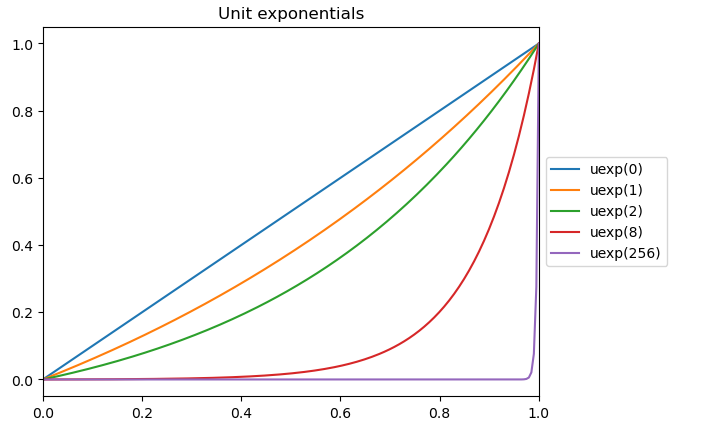
\includegraphics[width=\textwidth]{unit_exponentials.png}
\end{figure}

The most immediate advantage of unit exponentials is that they are all pinned to the $[0,1]$ interval:

\begin{equation}
\begin{array}{l}
\uexp{t}(0) = {{e^0 -1} \over {e^t - 1}} = 0\\
\uexp{t}(1) = {{e^t -1} \over {e^t - 1}} = 1\\
\end{array}
\end{equation}

This makes them extremely convenient for the problem of fitting absolutely monotonic functions $f:[0,1] \rightarrow [0,1]$. We note that $\lim\limits_{t \to 0} \uexp{t}(x) = x$, and so we can smoothly extend the definition to $\uexp{0}(x) = x$\\

However, their attractiveness only begins here. One of the most interesting properties of unit expontentials is that their value for any $x \in [0,1]$ always corresponds to the proportion of the total growth between $0$ and $1$ that {\emph{all}} of its derivatives have manifested between $0$ and $x$:

\begin{theorem}
For every $t > 0$, every $n \geq 0$, and every $x \in [0,1]$.
\begin{equation}
{{\nderiv{\uexp{t}}{n}(x) - \nderiv{\uexp{t}}{n}(0)} \over {\nderiv{\uexp{t}}{n}(1) - \nderiv{\uexp{t}}{n}(0)}} = \uexp{t}(x)
\end{equation}
\end{theorem}

While unit exponentials always go between 0 and 1, their derivatives do not necessarily do so. They are always greater than $0$ at $0$ and grow to very high values near $1$, with no bound for unbounded $t$. However, the theorem establishes a link between the function itself and how fast {\bf{all}} of the derivatives grow, displaying a very significant and regular coordination among all derivatives for unit exponentials.\\

There are two useful lemmas that we will use to prove this theorem among other things.

\begin{lemma}
For every $t > 0$ and $n > 0$,
\begin{equation}
\nderiv{\uexp{t}}{n}(x) = {{t^n e^{tx}} \over {e^t - 1}}
\end{equation}
\end{lemma}

\begin{proof}
This is a simple inductive application of the derivation of $\uexp{t}(x) = {{e^{tx} - 1} \over {e^t - 1}}$.
\end{proof}

\begin{lemma}
For every $t > 0$ and $n > 0$,
\begin{equation}
\begin{array}{l}
\nderiv{\uexp{t}}{n}(0) = {{t^n} \over {e^t - 1}}\\
\nderiv{\uexp{t}}{n}(1) = {{t^n e^t} \over {e^t - 1}}\\
\nderiv{\uexp{t}}{n}(1) - \nderiv{\uexp{t}}{n}(0) = t^n\\
\end{array}
\end{equation}
\end{lemma}

\begin{proof}
The first two lines are a direct application of the previous lemma, but we will write the derivation of the last line explicitly, as it is the most interesting part of this lemma, providing a direct expression for the range of the $n$-th derivative of $\uexp{t}$ depending cleanly on $t$.

\begin{equation}
\nderiv{\uexp{t}}{n}(1) - \nderiv{\uexp{t}}{n}(0) =  {{t^n e^t} \over {e^t - 1}} - {{t^n} \over {e^t - 1}} = {{t^n (e^t - 1)} \over {e^t -1}} = t^n
\end{equation}
\end{proof}

Note that his last line also holds for $n = 0$, that is, it is also the case that $\uexp{t}(1) - \uexp{t}(0) = t^0 = 1$.

We are now in a position to prove the theorem.

\begin{proof}[(Proof of the theorem)]
We first note that for $n = 0$ the theorem is trivial since $\uexp{t}(0) = 0$ and $\uexp{t}(1) - \uexp{t}(0) = 1$, so it follows directly from the equation.

\begin{equation}
{{\uexp{t}(x) - \uexp{t}(0)} \over {\uexp{t}(1) - \uexp{t}(0)}} = {{\uexp{t}(x) - 0} \over {1}} = \uexp{t}(x)
\end{equation}

For $n > 0$, we begin by simplifying the denominator to $t^n$ as per the lemma,

\begin{equation}
{{\nderiv{\uexp{t}}{n}(x) - \nderiv{\uexp{t}}{n}(0)} \over {\nderiv{\uexp{t}}{n}(1) - \nderiv{\uexp{t}}{n}(0)}} = {{\nderiv{\uexp{t}}{n}(x) - \nderiv{\uexp{t}}{n}(0)} \over {t^n}}
\end{equation}

We can then replace the two values in the numerator,

\begin{multline}
{{\nderiv{\uexp{t}}{n}(x) - \nderiv{\uexp{t}}{n}(0)} \over {t^n}} = {{1} \over {t^n}} \cdot ({{t^n e^{tx}} \over {e^t - 1}} - {{t^n} \over {e^t - 1}}) = \\
= {{1} \over {t^n}} \cdot {{t^n (e^{tx} - 1)} \over {e^t - 1}} = {{e^{tx} - 1} \over {e^t - 1}} = \uexp{t}(x)\\
\end{multline}
\end{proof}

By the middle point theorem, for any $t > 0$, there will always be a point $x_1(t) \in [0,1]$ where the first derivative of $\uexp{t}$ will be exactly 1. We will call this the {\emph{exploding point}} of $\uexp{t}$. All unit exponentials go underneath the straight line $\uexp{0}(x) = x$, with lower initial first derivative and higher final first derivative the higher the $t$. At some point, the first derivative will be exactly $1$, which can be identified to be as the point in which the unit exponential ``kicks off'' and begins its exponential growth. The location of the exploding point with respect to $t$ is interesting as it approximately separates the area where the unit exponential is flat and where it is steep. This point will always be $x_1(t) \geq 0.5$ for $t > 0$, and will get progressively closer to $1$ as $t$ increases. See figure \ref{fig_exploding_points} for a visualization of the exploding points of various unit exponentials.

It is, in fact, more interesting or useful to consider instead the distance between $x_1(t)$ and $1$. Write $1 - {\bar{x}}_1(t) = x_1(t)$. We can calculate this value analytically:

\begin{multline}
\uexp{t}^{\prime}(x_1(t)) = \uexp{t}^{\prime}(1 - {\bar{x}}_1(t)) = {{t e^{t (1 - {\bar{x}}_1(t))}} \over {e^t - 1}} = 1\\
t e^{t (1 - {\bar{x}}_1(t))} = e^t - 1\\
\ln t + t (1 - {\bar{x}}_1(t)) = \ln (e^t - 1)\\
1 - {\bar{x}}_1(t) = {{\ln (e^t - 1) - \ln t} \over {t}}\\
{\bar{x}}_1(t) = {{t + \ln t - \ln (e^t - 1)} \over {t}}\\
\end{multline}

\begin{figure}
\caption{\label{fig_exploding_points}Exploding points}
\centering
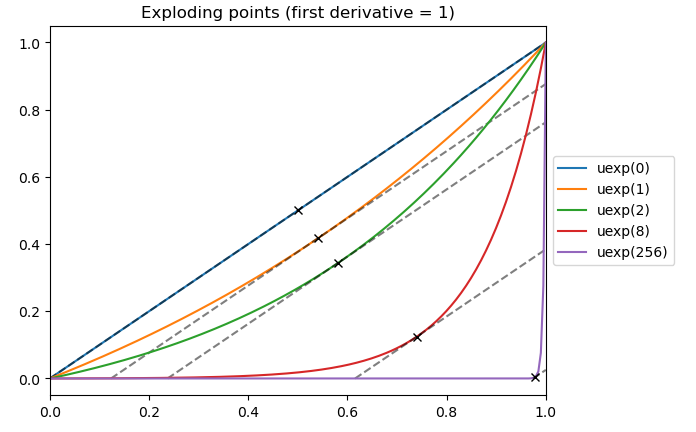
\includegraphics[width=\textwidth]{exploding_points.png}
\end{figure}

An interesting way to think about this gap between the exploding point and $1$ is to see how it changes when we multiply $t$ by a constant $k > 1$. Therefore, we can compare ${\bar{x}}_1(t)$ with ${\bar{x}}_1(kt)$. The latter will be smaller, as a larger $t$ moves the exploding point closer to $1$, but by how much? For large enough $t$, multiplying $t$ by $k > 1$ reduces the gap between the exploding point and $1$ to approximately $1/k$. That is, ${{{\bar{x}}_1(t)} \over {{\bar{x}}_1(kt)}} \simeq k$. This is very useful in the implementation of an iterative process to find a semiparametric fitting of an absolutely monotonic function as a sum of unit exponentials, as we can use a multiplying factor $k$ to obtain meaningful variation in the parameters of the unit exponentials that are independent of the current values of $t$ (see \S \ref{least_squares}).\\

We can show this numerically by plotting ${{{\bar{x}}_1(t)} \over {{\bar{x}}_1(kt)}}$ for various values of $k$. See figure \ref{fig_exploding_point_evolution}. Note that the convergence is notoriously slow (logarithmic), but it stabilises relatively quickly in a relatively constant range. It can be proven to be exactly $k$ in the limit (though this is not very useful because we will not use such large $t$).

\begin{figure}
\caption{\label{fig_exploding_point_evolution}Exploding point change when multiplying}
\centering
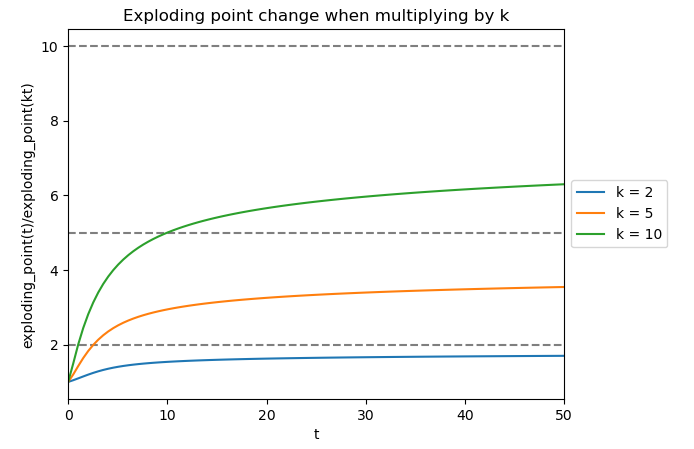
\includegraphics[width=\textwidth]{exploding_point_evolution.png}
\end{figure}

\begin{theorem}
\begin{equation}
\lim_{t \rightarrow \infty} {{{\bar{x}}_1(t)} \over {{\bar{x}}_1(kt)}} = k
\end{equation}
\end{theorem}

\begin{proof}
First note that

\begin{equation}
t - \ln(e^t - 1) = t - \ln(e^t(1 - e^{-t})) = t - t - \ln(1 - e^{-t}) = - \ln(1-e^{-t})
\end{equation}

With this in mind, simplify the original quotient.

\begin{multline}
{{{\bar{x}}_1(t)} \over {{\bar{x}}_1(kt)}} = {{t + \ln t - \ln(e^t - 1)} \over {kt + \ln kt - \ln(e^{kt} - 1)}} \cdot {{kt} \over {t}} =\\
k \cdot {{\ln t - \ln(1-e^{-t})} \over {\ln kt - \ln(1-e^{-kt})}} = k \cdot {{\ln t - \ln(1-e^{-t})} \over {\ln k + \ln t - \ln(1-e^{-kt})}}\\
\end{multline}

The latter terms go to 0 as $t \rightarrow \infty$, and so we have

\begin{equation}
\lim_{t \rightarrow \infty} {{{\bar{x}}_1(t)} \over {{\bar{x}}_1(kt)}} = \lim_{t \rightarrow \infty} k \cdot {{\ln t} \over {\ln k + \ln t}} = k \cdot 1 = k
\end{equation}
\end{proof}

One last but critical element to explain how we use unit exponentials to fit absolutely monotonic functions is to show how the Bernstein theorem (theorem \ref{bernstein_theorem}) applies to them.

\begin{theorem}
Let $\realfunction{f}{[0,1]}$ be an absolutely monotonic function. Then, there is a non-negative finite Borel measure $\mu$ such that
\begin{equation}
f(x) - f(0) = \int_{0}^{\infty} \uexp{t}(x) d \mu(t)
\end{equation}

\noindent for every $x \in [0,1]$
\end{theorem}

\begin{proof}
Start from Bernstein's theorem. Then there exists a non-negative finite Borel measure $\mu$ such that $f(x) = \int_{0}^{\infty} e^{tx} d \mu(t)$. But then,

\begin{multline}
f(x) = \int_{0}^{\infty} e^{tx} d \mu(t) = \int_{0}^{\infty} (e^{tx} - 1 + 1) d \mu(t) = \int_{0}^{\infty} (e^{tx} - 1) d \mu(t) + \int_{0}^{\infty} 1 d \mu(t) =\\
= \int_{0}^{\infty} (e^t - 1) {{e^{tx} - 1} \over {e^t - 1}} d \mu(t) + \int_{0}^{\infty} 1 d \mu(t)\\
\end{multline}

Since $e^t - 1$ is non-negative and integrable, we can define the non-negative finite Borel measure $d \nu(t) = (e^t - 1) d \mu(t)$ that is absolutely continuous with respect to $\mu$, and write:

\begin{equation}
f(x) =  \int_{0}^{\infty} {{e^{tx} - 1} \over {e^t - 1}} d \nu(t) + \int_{0}^{\infty} 1 d \mu(t) = \int_{0}^{\infty} \uexp{t}(x) d \nu(t) + \int_{0}^{\infty} 1 d \mu(t)
\end{equation}

Now consider 
\begin{equation}
f(0) =  \int_{0}^{\infty} \uexp{t}(0) d \nu(t) + \int_{0}^{\infty} 1 d \mu(t) = 0 + \int_{0}^{\infty} 1 d \mu(t) = \int_{0}^{\infty} 1 d \mu(t)
\end{equation}

\noindent and so

\begin{equation}
f(x) - f(0) = \int_{0}^{\infty} \uexp{t}(x) d \nu(t) + \int_{0}^{\infty} 1 d \mu(t) - \int_{0}^{\infty} 1 d \mu(t) = \int_{0}^{\infty} \uexp{t}(x) d \nu(t)
\end{equation}
\end{proof}

We can therefore attempt to approximate any absolutely monotonic function $f$ for which $f(0) = 0$ with a finite weighted sum of unit exponentials. Our goal now becomes, given the normalized dataset $\mathcal{D}$ with all x values in $[0,1]$, find a finite weighted sum of unit exponentials that explains the values in $\mathcal{D}$ as well as possible. By construction, this finite weighted sum will be absolutely monotonic, and because of the theorem, we know that if we use a large enough number of well selected unit exponentials, we should be able to approximate the values as well as any absolutely monotonic function could.

\subsection{Least squares optimization}
\label{least_squares}

\subsection{Evaluation}

\section{Results}

\section{Conclusions}

\dobibliography

\end{document}